\chapter{VHash And DGVH}
\label{chapter:dgvh}
DHTs all seek to minimize lookup time for their respective topologies.
This is done by minimizing the number of overlay hops needed for a lookup operation.
This is a good approximation for minimizing the latency of lookups, but does not actually do so, as each hop has a different amount of latency.
Furthermore, a network might need to minimize some arbitrary metric, such as energy consumption.

VHash is a multi-dimensional DHT that minimizes routing over some given metric.
It uses a fast approximation of a Delaunay Triangulation to compute the Voronoi tessilation of a multi-dimensional space.
%Approximated routing tables



Arguably all Distributed Hash Tables (DHTs) are built on the concept of Voronoi tessellations.
In all DHTs, a node is responsible for all points in the overlay to which it is the ``closest'' node.
Nodes are assigned a key as their location in some keyspace, based on the hash of certain attributes.
Normally, this is just the hash of the IP address (and possibly the port) of the node \cite{chord} \cite{kademlia} \cite{can} \cite{pastry}, but other metrics such as geographic location can be used as well \cite{ratnasamy2002ght}.

These DHTs have carefully chosen metric spaces such that these regions are very simple to calculate.
For example, Chord \cite{chord} and similar ring-based DHTs \cite{symphony} utilize a unidirectional, one-dimensional ring as their metric space, such that the region for which a node is responsible is the region between itself and its predecessor.

Using a Voronoi tessellation in a DHT generalizes this design.
Nodes are Voronoi generators at a position based on their hashed keys.
These nodes are responsible for any key that falls within its generated Voronoi region.

Messages get routed along links to neighboring nodes.
This would take $O(n)$ hops in one dimension.
In multiple dimensions, our routing algorithm (Algorithm \ref{alg:lookup}) is extremely similar to the one used in Ratnasamy et al.'s Content Addressable Network (CAN) \cite{can}, which would be $O(n^{\frac{1}{d}})$ hops.


\begin{algorithm}
	\caption{Lookup in a Voronoi-based DHT}
	\label{alg:lookup}
	\begin{algorithmic}[1]
		\State Given node $n$
		\State Given $m$ is a message addressed for $loc$
		\State $potential\_dests \leftarrow n \cup n.short\_peers \cup n.long\_peers$
		\State $c \leftarrow $ node in $ potential\_dests$ with shortest distance to $loc$
		\If{$c$ == $n$}
			\State \Return $n$
		\Else
			\State \Return $c.lookup(loc)$
		\EndIf
	\end{algorithmic}
\end{algorithm}


Efficient solutions, such as Fortune's sweepline algorithm \cite{fortune1987sweepline}, are not usable in spaces with 2 more dimensions.
As far as we can tell, there is no way efficient to generate higher dimension Voronoi tessellations, especially in the distributed Churn-heavy context of a DHT.
Our solution is the Distributed Greedy Voronoi Heuristic.

\section{Distributed Greedy Voronoi Heuristic}
A Voronoi tessellation is the partition of a space into cells or regions along a set of objects $O$, such that all the points in a particular region are closer to one object than any other object.
We refer to the region owned by an object as that object's Voronoi region.
Objects which are used to create the regions are called Voronoi generators.
In network applications that use Voronoi tessellations, nodes in the network act as the Voronoi generators.

The Voronoi tessellation and Delaunay triangulation are dual problems, as an edge between two objects in a Delaunay triangulation exists if and only if those object's Voronoi regions border each other.
This means that solving either problem will yield the solution to both.
An example Voronoi diagram is shown in Figure \ref{voro-ex}.
For additional information, Aurenhammer \cite{voronoi} provides a formal and extremely thorough description of Voronoi tessellations, as well as their applications.


\begin{figure}
	\centering
	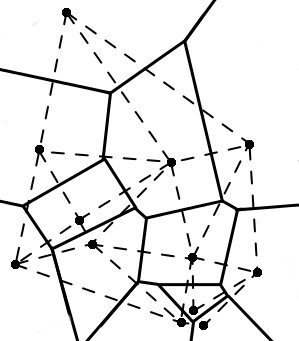
\includegraphics[width=0.5\linewidth]{figs/voronoi}
	\caption{An example Voronoi diagram for objects on a 2-dimensional space.  The black lines correspond to the borders of the Voronoi region, while the dashed lines correspond to the edges of the Delaunay Triangulation.}
	\label{voro-ex}
\end{figure}




The Distributed Greedy Voronoi Heuristic (DGVH) is a fast method for nodes to define their individual Voronoi region (Algorithm \ref{alg:dgvh}).
This is done by selecting the nearby nodes that would correspond to the points connected to it by a Delaunay triangulation.
The rationale for this heuristic is that, in the majority of cases, the midpoint between two nodes falls on the common boundary of their Voronoi regions.

%In addition, nodes should only have to compute their own Voronoi region, and possibly estimate those of its neighbors.
%Anything else is a waste of processing power.



\begin{algorithm} % make smaller
	\caption{Distributed Greedy Voronoi Heuristic}
	\label{alg:dgvh}
	\begin{algorithmic}[1]  % the numberis how many lines
		\State Given node $n$ and its list of $candidates$.
		\State Given the minimum $table\_size$
		\State $short\_peers \leftarrow$ empty set that will contain $n$'s one-hop peers
		\State $long\_peers \leftarrow$ empty set that will contain $n$'s two-hop peers
		\State Sort $candidates$ in ascending order by each node's distance to $n$
		\State Remove the first member of $candidates$ and add it to $short\_peers$
		\ForAll{$c$ in $candidates$}
		\State $m$ is the midpoint between $n$ and $c$
		\If{Any node in $short\_peers$ is closer to $m$ than $n$}
		\State Reject $c$ as a peer
		\Else
		\State Remove $c$ from $candidates$
		\State Add $c$ to $short\_peers$
		\EndIf
		\EndFor
		\While{$|short\_peers| < table\_size$ \textbf{and} $|candidates| >0$}
		\State Remove the first entry $c$ from $candidates$
		\State Add $c$ to $short\_peers$
		\EndWhile
		\State Add $candidates$ to the set of $long\_peers$
		\If{$|long\_peers| > table\_size^2$}
		\State $long\_peers \leftarrow$ random subset of $long\_peers$ of size $table\_size^2$
		\EndIf
	\end{algorithmic}
\end{algorithm}


During each cycle, nodes exchange their peer lists with a current neighbor and then recalculate their neighbors.
A node combines their neighbor's peer list with its own to create a list of candidate neighbors.
This combined list is sorted from closest to furthest.
A new peer list is then created starting with the closest candidate.
The node then examines each of the remaining candidates in the sorted list and calculates the midpoint between the node and the candidate.
If any of the nodes in the new peer list are closer to the midpoint than the candidate, the candidate is set aside.
Otherwise the candidate is added to the new peer list.


DGVH never actually solves for the actual polytopes that describe a node's Voronoi region.
This is unnecessary and prohibitively expensive \cite{raynet}.
Rather, once the heuristic has been run, nodes can determine whether a given point would fall in its region.

Nodes do this by calculating the distance of the given point to itself and other nodes it knows about.
The point falls into a particular node's Voronoi region if it is the node to which it has the shortest distance.
This process continues recursively until a node determines that itself to be the closest node to the point.
Thus, a node defines its Voronoi region by keeping a list of the peers that bound it.



\subsection{Algorithm Analysis}

DVGH is very efficient in terms of both space and time.
Suppose a node $n$ is creating its short peer list from $k$ candidates in an overlay network of $N$ nodes.
The candidates must be sorted, which takes $O(k\cdot\lg(k))$ operations.
Node $n$ must then compute the midpoint between itself and each of the $k$ candidates.
Node $n$ then compares distances to the midpoints between itself and all the candidates.
This results in a cost of

\[ k\cdot\lg(k) + k \text{ midpoints}  + k^{2} \text{ distances} \]


Since $k$ is  bounded by $\Theta(\frac{\log N}{\log \log N} )$ \cite{bern1991expected} (the expected maximum degree of a node), we can translate the above to

\[O(\frac{\log^{2} N}{\log^{2} \log N} )\]

In the vast majority of cases, the number of peers is equal to the minimum size of \textit{Short Peers}.
This yields $k=(3d+1)^{2}+3d+1$ in the expected case, where the lower bound and expected complexities are $\Omega(1)$.



\section{Experimental Results}
We evaluated the effectiveness of VHash and DGVH in creating a set of experiments.\footnote{Our results are pulled directly from \cite{dgvh} and \cite{vhash}.}
The first experiment showed how VHash could use DGVH to create a routing mesh.
Our second showed how optimizing for latency yielded better results than optimizing for least hops.

\subsection{Convergence}
Our first experiment examined how DGVH could be used to create a routing overlay and how well it performed in this task.
The simulation demonstrated how DGVH  formed a stable overlay from a chaotic starting topology after a number of cycles.
We compared our results to those in RayNet \cite{raynet}.
The authors of Raynet proposed a random $k$-connected graph would be a challenging initial configuration for showing a DHT relying on a gossip mechanism could converge to a stable topology.

In the initial two cycles of the simulation, each node bootstrapped its short peer list by appending 10 nodes, selected uniformly at random from the entire network.
In each cycle, the nodes gossiped , swapping peer list information.
They then ran DGVH using the new information.
We calculated the hit rate of successful lookups by simulating 2000 lookups from random nodes to random locations, as described in Algorithm \ref{alg:routesim}.
A lookup was considered successful if the network was able to determine which Voronoi region contained a randomly selected point.

Our experimental variables for this simulation were the number of nodes in the DGVH generated overlay and the number of dimensions.
We tested network sizes of 500, 1000, 2000, 5000, and 10000 nodes each in 2, 3, 4, and 5 dimensions.
The hit rate at each cycle is $\frac{hits}{2000}$, where $hits$ are the number of successful lookups.




\begin{algorithm}
	\caption{Routing Simulation Sample}
	\label{alg:routesim}
	\begin{algorithmic}[1]  % the number is how many
		\State $start \leftarrow$ random node
		\State$dest \leftarrow$ random set of coordinates
		\State $ans \leftarrow$ node closest to $dest$
		\If {$ans == start.lookup(dest)$}
		\State increment $hits$
		\EndIf
	\end{algorithmic}
\end{algorithm}

The results of our simulation are shown in Figure \ref{fig:conv}.
Our graphs show that a correct overlay was quickly constructed from a random configuration and that our hit rate reached 90\% by cycle 20, regardless of the number of dimensions.
Lookups consistently approached a hit rate of 100\% by cycle 30.
In comparison, RayNet's routing converged to a perfect hit rate at around cycle 30 to 35 \cite{raynet}.
As the network size and number of dimensions each increase, convergence slows, but not to a significant degree.

\begin{figure*}
	\centering
	\begin{tabular}{cc}

		\begin{subfigure}{0.5\columnwidth}
			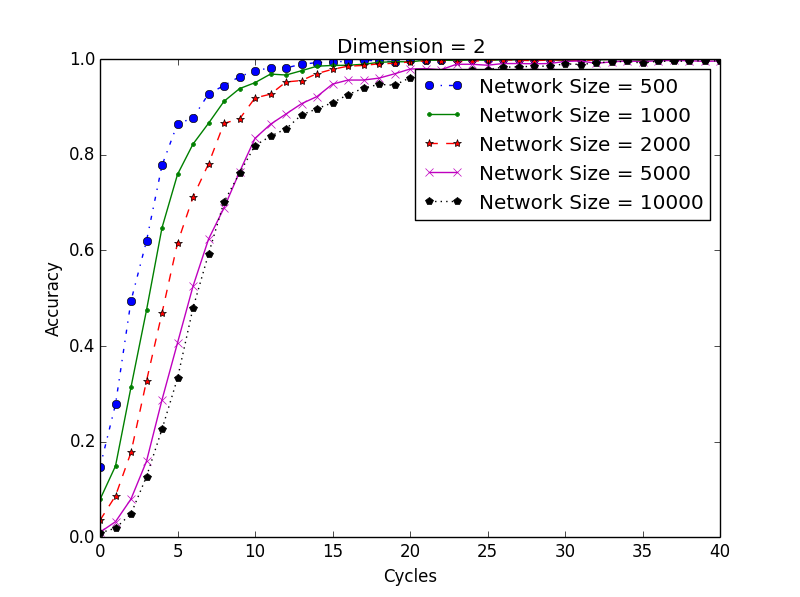
\includegraphics[width=\linewidth]{figs/conv_d2}
			\caption{This plot shows the accuracy rate of lookups on a 2-dimensional network as it self-organizes.}
			\label{fig:conv2}
		\end{subfigure} &

		\begin{subfigure}{0.5\columnwidth}
			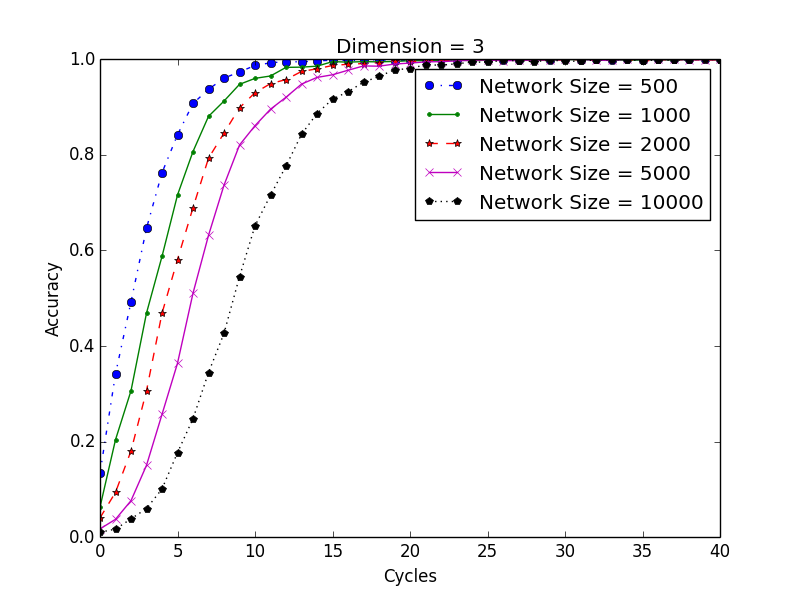
\includegraphics[width=\linewidth]{figs/conv_d3}
			\caption{This plot shows the accuracy rate of lookups on a 3-dimensional network as it self-organizes.}
			\label{fig:conv3}
		\end{subfigure} \\

		\begin{subfigure}{0.5\columnwidth}
			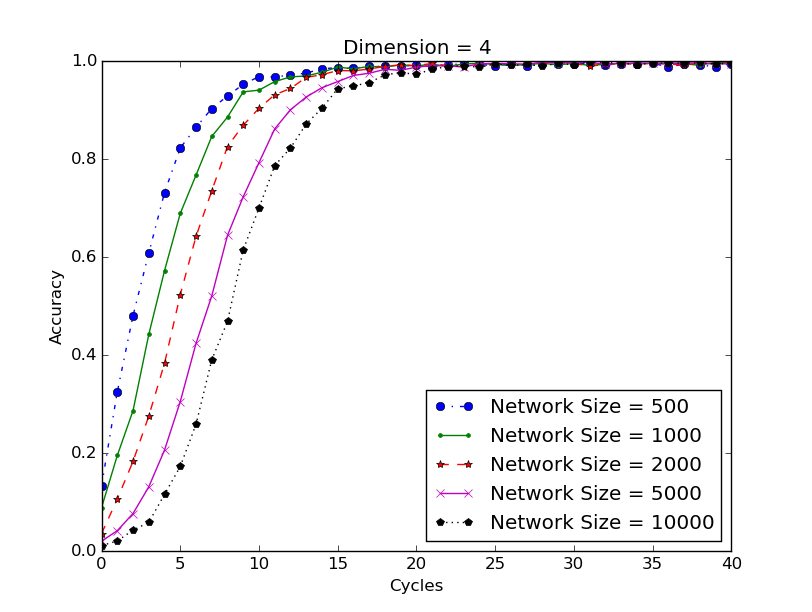
\includegraphics[width=\linewidth]{figs/conv_d4}
			\caption{This plot shows the accuracy rate of lookups on a 4-dimensional network as it self-organizes.}
			\label{fig:conv4}
		\end{subfigure} &


		\begin{subfigure}{0.5\columnwidth}
			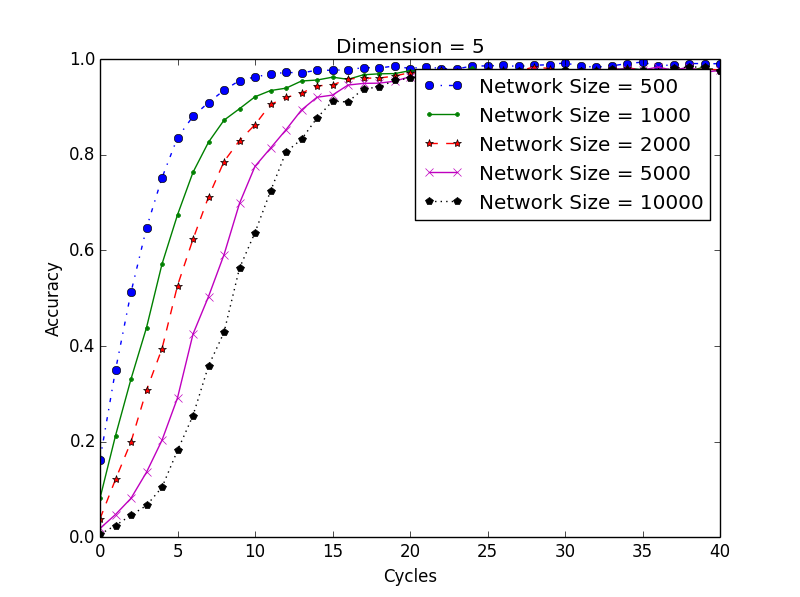
\includegraphics[width=\linewidth]{figs/conv_d5}
			\caption{This plot shows the accuracy rate of lookups on a 5-dimensional network as it self-organizes.}
			\label{fig:conv5}
		\end{subfigure}

	\end{tabular}
	\caption{These figures show that, starting from a randomized network, DGVH forms a stable and consistent network topology.
		The Y axis shows the success rate of lookups and the X axis show the number of gossips that have occurred.
		Each point shows the fraction of 2000 lookups that successfully found the correct destination.}
	
	\label{fig:conv}

\end{figure*}

\subsection{Latency Distribution Test}
The goal of our second set of experiments was to demonstrate VHash's ability to optimize a selected network metric: latency in this case.
In our simulation, we used the number of hops on the underlying network as an approximation of latency.
We compared VHash's performance to Chord \cite{chord}.
As we discussed in Chapter \ref{chapter:background} Chord is a well established DHT with an $O(\log(n))$ sized routing table and $O(\log(n))$ lookup time measured in overlay hops.

Instead of using the number of hops on the overlay network as our metric, we are concerned with the actual latency lookups experience traveling through the \emph{underlay} network, the network upon which the overlay is built.
Overlay hops are used in most DHT evaluations as the primary measure of latency.
It is the best approach available when there are no means of evaluating the characteristics of the underlying network.
VHash is designed with a capability to exploit the characteristics of the underlying network.
With most realistic network sizes and structures, there is substantial room for latency reduction in DHTs.

For this experiment, we constructed a scale free network with 10000 nodes placed at random (which has an approximate diameter of 3 hops) as an underlay network \cite{cohen2000resilience} \cite{pastor2001epidemic} \cite{hagberg2004}.
We chose to use a scale-free network as the underlay, since  scale free networks model the Internet's topology \cite{cohen2000resilience} \cite{pastor2001epidemic}.
We then chose a random subset of nodes to be members of the overlay network.
Our next step was to measure the distance in underlay hops between 10000 random source-destination pairs in the overlay.
VHash generated an embedding of the latency graph utilizing a distributed force directed model, with the latency function defined as the number of underlay hops between it and its peers.

Our simulation created 100, 500, and 1000 node overlays for both VHash and Chord.
We used 4 dimensions in VHash and a standard 160 bit identifier for Chord.




\begin{figure}

\begin{subfigure}{\columnwidth}
\centering
	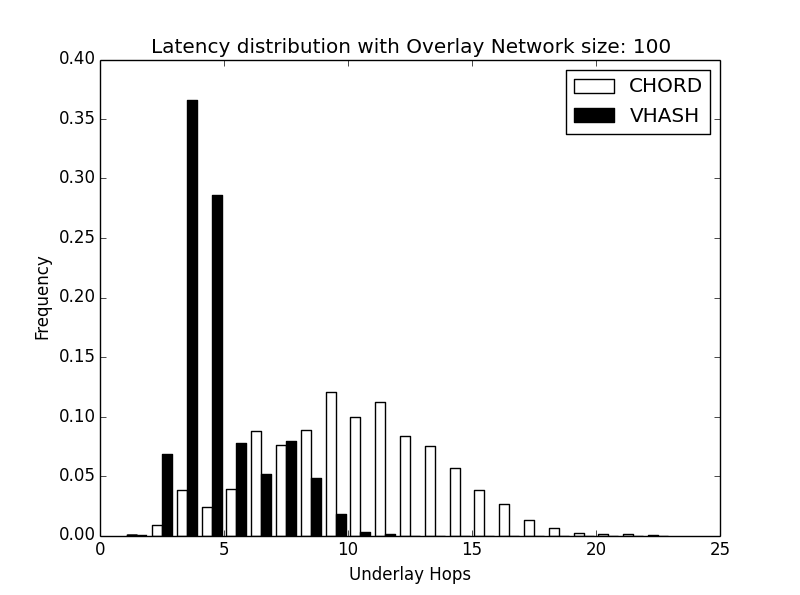
\includegraphics[width=0.5\linewidth]{figs/hist_100}
	\caption{Frequency of path lengths on Chord and VHash in a 100 node overlay.}
	\label{fig:hist100}
\end{subfigure}

\begin{subfigure}{\columnwidth}
	\centering
	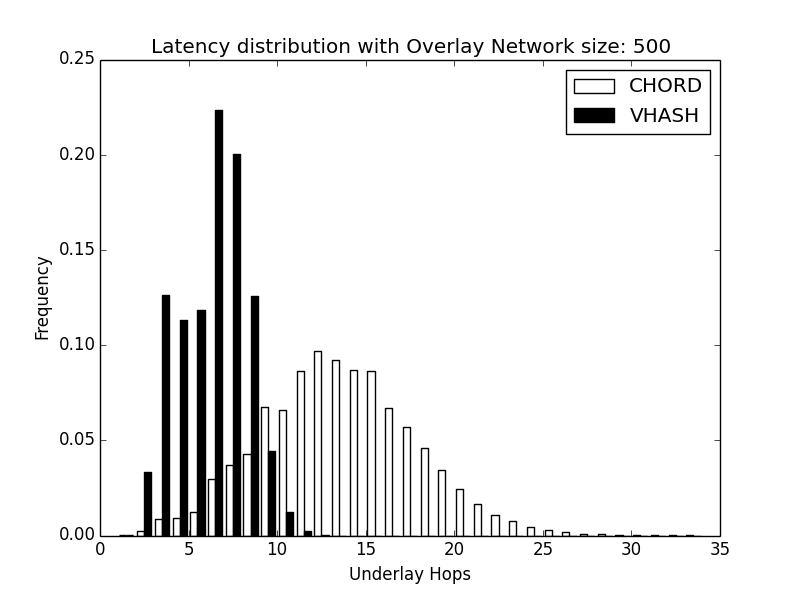
\includegraphics[width=0.5\linewidth]{figs/hist_500}
	\caption{Frequency of path lengths on Chord and VHash in a 500 node overlay.}
	\label{fig:hist500}
\end{subfigure}

\begin{subfigure}{\columnwidth}
	\centering
	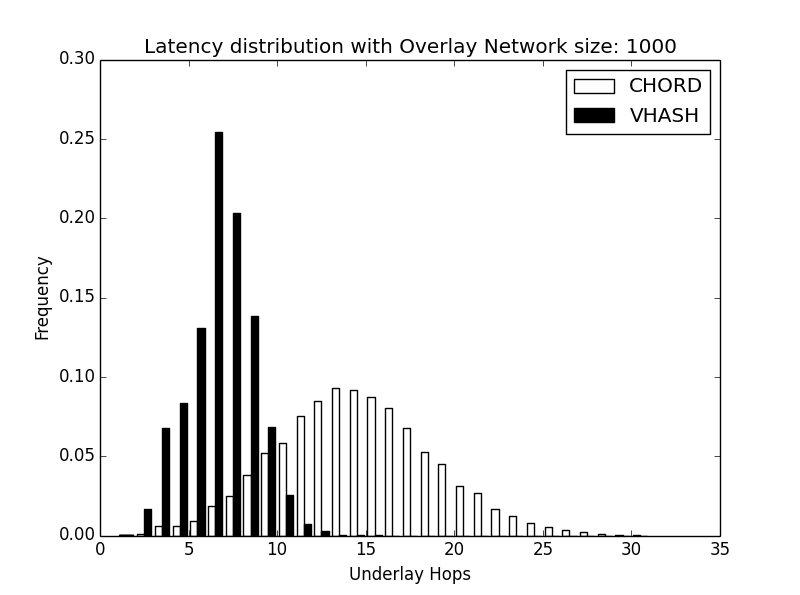
\includegraphics[width=0.5\linewidth]{figs/hist_1000}
	\caption{Frequency of path lengths on Chord and VHash in a 1000 node overlay.}
	\label{fig:hist1000}
\end{subfigure}

\caption{Figures \ref{fig:hist100}, \ref{fig:hist500}, and \ref{fig:hist1000} show the difference in the performance of Chord and VHash for 10,000 routing samples on a 10,000 node underlay network for differently sized overlays.
The Y axis shows the observed frequencies and the X axis shows the number of hops traversed on the underlay network.
VHash consistently requires fewer hops for routing than Chord.}
\label{fig:hist}

\end{figure}




Figure \ref{fig:hist} shows the distribution of path lengths measured in underlay hops in both Chord and VHash.
VHash significantly outperformed Chord and considerably reduced the underlay path lengths in three network sizes.

We also sampled the lookup length measured in overlay hops for a 1000 sized Chord and VHash network.
As seen in Figure \ref{fig:histover}, the paths measured in overlay for VHash were significantly shorter than those in Chord.
In comparing the overlay and underlay hops, we find that for each overlay hop in Chord, the lookup must travel 2.719 underlay hops on average; in VHash, lookups must travel 2.291 underlay hops on average for every overlay hop traversed.

Recall that this work is based on scale free networks, where latency improvements are difficult.
An improvement of 0.4 hops over a diameter of 3 hops is significant.
VHash has on average less overlay hops per lookup than Chord, and for each of these overlay hops we consistently traverse more efficiently across the underlay network.
\begin{figure}
	\centering
	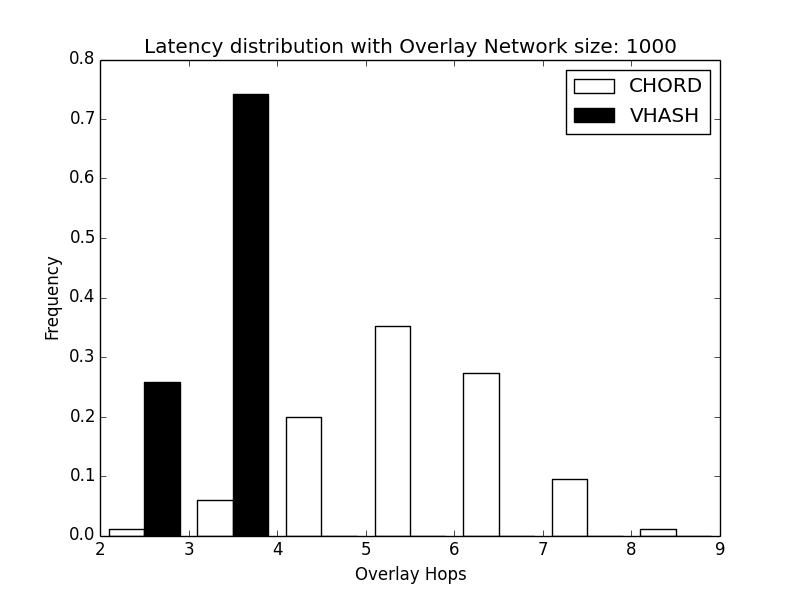
\includegraphics[width=0.5\linewidth]{figs/hist_overlay_4d}
	\caption{Comparison of Chord and VHash in terms of overlay hops.  Each overlay has 1000 nodes.  The Y axis denotes the observed frequencies of overlay hops and the X axis corresponds to the path lengths in overlay hops.}
	\label{fig:histover}
\end{figure}




\section{Remarks}

Voronoi tessellations have a wide potential for applications in ad-hoc networks, massively multiplayer games, P2P, and distributed networks.
However, centralized algorithms for Voronoi tessellation and Delaunay triangulation are not applicable to decentralized systems.
In addition, solving Voronoi tessellations in more than 2 dimensions is computationally expensive.

We created a distributed heuristic for Voronoi tessellations in an arbitrary number of dimensions.
Our heuristic is fast and scalable, with a expected memory cost of $(3d+1)^{2}+3d+1$ and expected maximum runtime of O$(\frac{\log^{2} N}{\log^{2} \log N} )$.

We ran two sets of experiments to demonstrate VHash's effectiveness.
Our first set of experiments demonstrated that our heuristic is reasonably accurate  and our second set demonstrates that reasonably accurate is sufficient to build a P2P network which can route accurately.
Our second experiment showed that VHash  could significantly reduced the latency in Distributed Hash Tables.
